% 开普勒第一定律的证明
% 开普勒第一定律|圆锥曲线轨道|LRL矢量|比耐公式

\pentry{开普勒三定律\upref{Keple}}

\subsection{结论}
行星轨道是以中心天体为焦点的任意圆锥曲线\footnote{所以行星轨道不一定是椭圆, 也可以是抛物线或者双曲线, 但是抛物线或双曲线轨道是从无穷远来到无穷远去的轨道, 不会绕中心天体旋转. 所以开普勒定律作为行星运动的经验公式,只描述了椭圆.}.极坐标中,圆锥曲线的方程\upref{Cone}
为
\begin{equation}\label{Keple1_eq1}
r = \frac{p}{1 - e \cos \theta }
\end{equation}
令太阳中心天体在坐标原点,则行星沿该轨道运行.

\subsection{证明(LRL 矢量)}
\pentry{拉普拉斯—龙格—楞次矢量\upref{LRLvec}}

我们先来看一种无需微分方程的推导, 将开普勒问题中的 LRL 矢量 $\bvec A$ 内积位矢 $\bvec r$ 得
\begin{equation}\label{Keple1_eq2}
\bvec A \vdot \bvec r = (\bvec p \cross \bvec L)\vdot \bvec r - mkr
\end{equation}
由矢量混合积公式\autoref{TriVM_eq1}~\upref{TriVM}, 右边第一项为
\begin{equation}
(\bvec p \cross \bvec L)\vdot \bvec r = (\bvec r \cross \bvec p)\vdot \bvec L = L^2
\end{equation}
令 $\theta$ 为从 $\uvec A$ 转向 $\uvec r$ 的夹角(令极轴与矢量 $\bvec A$ 平行,如\autoref{Keple1_fig1}),则\autoref{Keple1_eq2} 变为
\begin{figure}[ht]
\centering
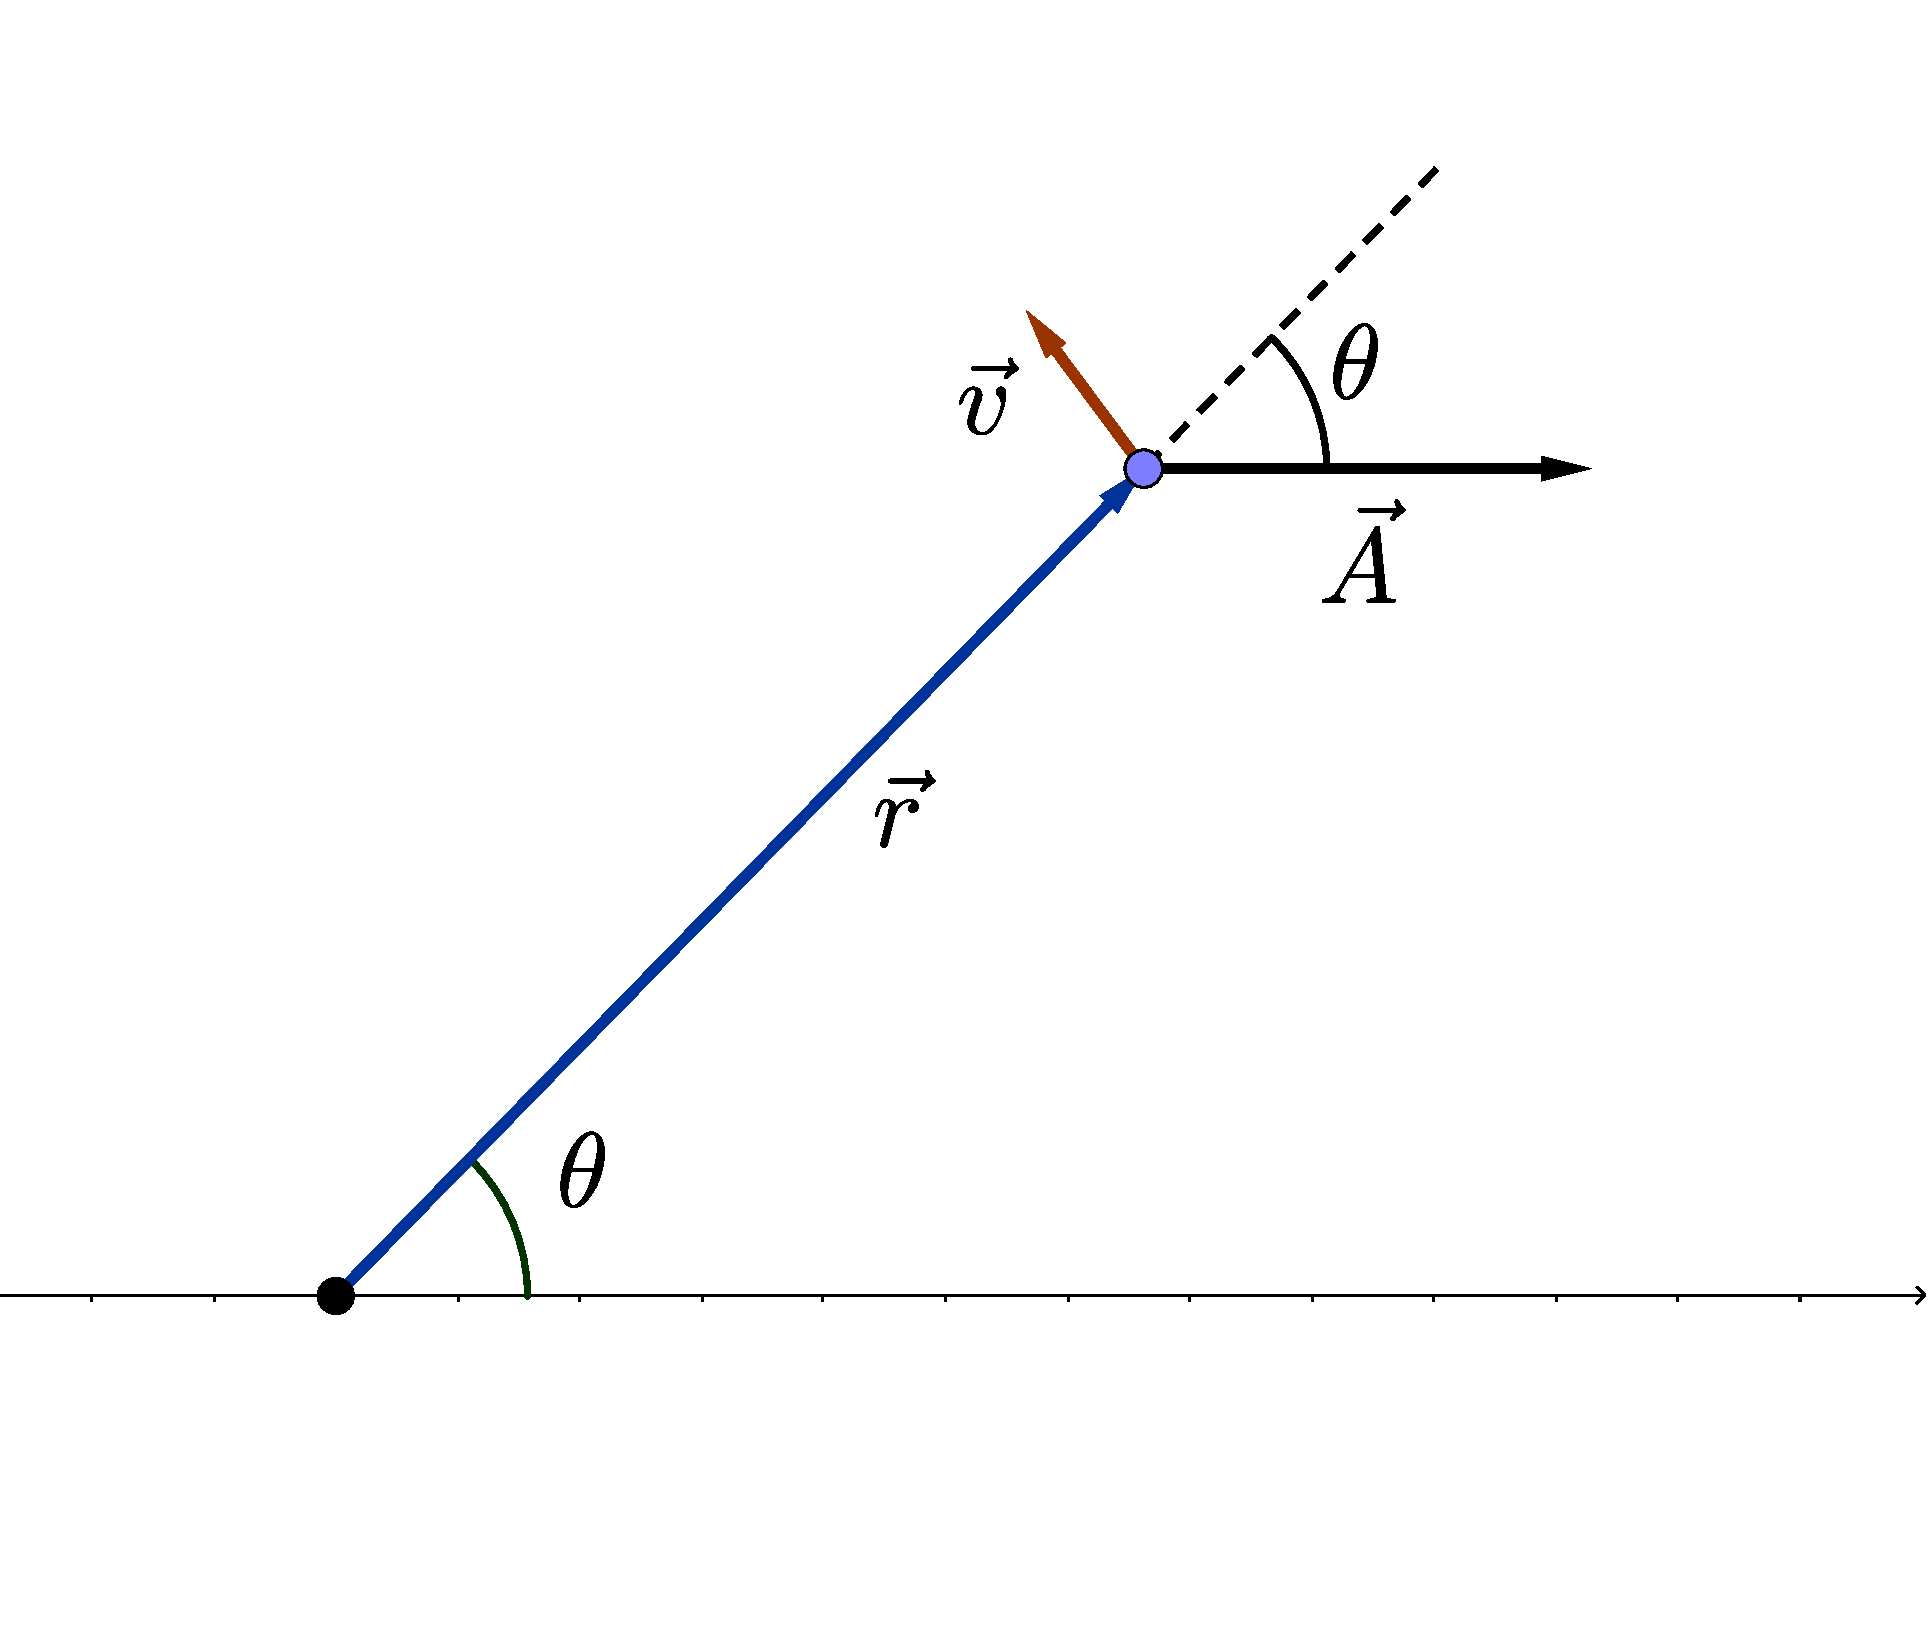
\includegraphics[width=6cm]{./figures/Keple1_1.pdf}
\caption{LRL矢量与位置矢量夹角} \label{Keple1_fig1}
\end{figure}
\begin{equation}
Ar\cos\theta = L^2 - mkr
\end{equation}
可得极坐标中的轨道为圆锥曲线的极坐标方程\footnote{对比\autoref{Keple1_eq1} 会发现分母的正负号反了, 这相当于把圆锥曲线旋转了 $180^\circ$,并不影响形状.}
\begin{equation}
r(\theta) = \frac{p}{1 + e\cos\theta}
\end{equation}
其中通径为 $p = L^2/(mk)$, 离心率为 $e = A/(mk)$.

\subsection{证明(比耐公式)}
\pentry{比耐公式\upref{Binet}, 二阶常系数非齐次微分方程的通解\upref{Ode2N}}

将平方反比力 $F(r) = -k/r^2$ 即 $F(1/u) = -ku^2$ 代入比耐公式
\begin{equation}
\dv[2]{u}{\theta} + u = -\frac{m}{L^2 u^2} F\qty(\frac 1u)
\end{equation}
通解\upref{Ode2N}为
\begin{equation}\label{Keple1_eq7}
u(\theta) = \frac{1}{p} \qty[1 - e\cos(\theta  + \phi_0)]
\end{equation}
其中
\begin{equation}
p = \frac{L^2}{mk}
\end{equation}
将\autoref{Keple1_eq7} 代入 $r = 1/u$, 得到圆锥曲线\autoref{Keple1_eq1}. 证毕.
